% ============================
% please see
% http://scc.stat.ucla.edu/mini-courses
% for additional information,
% mini-course schedules, or
% the accompanying
% presentation
% ============================

\documentclass[11pt]{article} % 'article' is the document type while '11pt' is an optional argument. there are many document types, and there are many potential options to include for each document type.

\usepackage{geometry}
\geometry{letterpaper}     % ... or a4paper or a5paper or ... 
\usepackage{graphicx}
\usepackage{amssymb}
\usepackage{epstopdf}
\usepackage{amsmath}  % this permits text in eqnarray among other benefits
\usepackage{color}          % gives color options
%\usepackage{fullpage} % this package makes use of more of each page but is not always installed
\usepackage{natbib}

\DeclareGraphicsRule{.tif}{png}{.png}{`convert #1 `dirname #1`/`basename #1 .tif`.png}

\title{LaTeX Examples}
\author{David Diez \\
UCLA Statistical Consulting Center}
\date{}  % removing the comment makes it produce no date

\begin{document} % this is the formal beginning of the document. the stuff above essentially preloads files and gets prior info.
\maketitle % don't want a title, author, or date listed? comment out this line.
\tableofcontents % compile twice to have the TOC up to date; comment this line out for no TOC
%\setlength{\parindent}{0in} % activate this to have no paragraph indentation
\pagebreak

It is assumed the reader is viewing both the document \texttt{latexTemp.tex} and \texttt{latexTemp.pdf} simultaneously to become familiar with how to control the text. Also reviewing the accompanying presentation is highly recommended.

\section{General}

\subsection{Header section}



Often times this part of the LaTeX document can be ignored, with the exception of the \texttt{$\backslash$title}, \texttt{$\backslash$author}, and \texttt{$\backslash$date}. Always update the title, author, and possibly also the date, otherwise comment out the \texttt{$\backslash$maketitle} command. See the presentation slides for additional details.

\subsection{Outline}
The section and subsection commands are used to make the sections and headers. For example, ``General'' is a section, and ``Header section'' and ``Outline'' are subsections.

\subsection{Paragraphs}

A new paragraphs can be created simply by creating two blank lines between between the text. For instance, this paragraph is ended by hitting ``enter'' twice (see the .tex document)...
This is not a new paragraph...

But this is a new paragraph. If an extra space is desired between paragraphs, use the double-backslash command and hit ``enter'' twice... \\

The PDF will now insert a space between the last paragraph and this one. \\

\noindent To make a particular paragraph have no indentation, use the command \texttt{$\backslash$noindent}, as in this paragraph. \\




Generally, lots of extra spaces won't           affect      		 	    the output text     in    the PDF. A new page can be created using the command \texttt{$\backslash$pagebreak}.

\pagebreak

\subsection{Spacing}
\label{spacing}

Horizontal text can be inserted in text using the \texttt{$\backslash$hspace\{0.3cm\}} \hspace{0.3cm} command. The argument in the command can be changed, of course, to be larger or smaller, i.e. it can be 0.1cm, 2.5cm, 1.3in, etc. The command \texttt{$\backslash$vspace\{1.1cm\}} \\
\vspace{1.1cm}

\noindent works in a similar way. LaTeX will accept specified lengths in \texttt{cm}, \texttt{mm}, \texttt{in}, among a few other options.

\subsection{Text}

Text can also be manipulated using commands. For example, use the command \texttt{$\backslash$emph} to \emph{emphasize} (italicize) text. {\em There are a few ways to italicize text.} \{Braces\} are often used to capture what the command acts on. Similar to italicizing, text can also be \textbf{bolded} in {\bfseries multiple ways} or text can be {\color{red} colored}. You can even create your own colors...
\definecolor{myRed}{rgb}{.7,.2,.1} % the 1st number says how much red, the 2nd green, the 3rd blue
{\color{myRed}this is ``myRed''}. % the package ``color'' must be included to do colors.
You can also \texttt{type like a typewriter}. \\

Using the shift-apostrophe key to get "double quotes" doesn't look very pretty in LaTeX. Instead, double the apostrophe up by the ``1 key'' for the ``left quote and use the double quotes" for the right quote. \\

Text can also be made {\tiny tiny}, {\scriptsize scriptsize}, {\footnotesize footnotesize}, {\small small}, {\large large}, {\Large Large}, {\LARGE LARGE}, etc. \\

\subsection{Macros}

In general, the commands used in this section can be found using the \textbf{Macros}. For example, to get the font size that you want in TeXShop, go to Macros $>$ Text Styles $>$ size. Also, try out quotations (Macros $>$ Insertions $>$ quotation:
\begin{quotation} %\em % perhaps you want it italicized?
This could be a very long quotation that you would not normally like to include in a paragraph. So instead you want it to stand alone and have a smaller width than a normal paragraph. This particular text was could easily be italicized using $\backslash$em at the start of the quotation, if desired.
\end{quotation}

\subsection{Lists}

The three preceding subsections are...
\begin{itemize}
\item Spacing
\item Text
\item Macros
\end{itemize}
Lists use the \texttt{itemize} environment or, if you want things numbered, \texttt{enumerate}:
\begin{enumerate}
\item Spacing
\item Text
\item Macros
\end{enumerate}
But the numbers should match the subsection names and there are options to do that, too...
\begin{enumerate}
\item[\ref{spacing}] Spacing % ref{} will be explained in the Tables section.
\item[1.5] Text
\item[1.6] Macros
\end{enumerate}

\subsection{Special characters}

LaTeX code uses a lot of special characters, which means if you want to put these characters in your text, you must \emph{escape} the characters from their usual purpose. For instance, each of the following commands requires a backslash to precede them to show up: \#, \$, \{, \}, \&, \%, \_. $\backslash$ and $\sim$ take a little more fussing. Greek letters and symbols will be introduced in Section~\ref{math}.

\subsection{verbatim}

When you really need to put text out explicitly, use verbatim:
\begin{verbatim}
All this stuff looks just like it \emph{would} if
you looked in the LaTeX file. % and comments don't work in verbatim...
\end{verbatim}

\section{Tabbing}
\label{tabbing}

\subsection{Basic tabbing}

Text can be indented using the indent command: \\
\indent\indent\indent This is indented text. \\

More importantly, custom tabbing can be created. For example
\begin{tabbing}
First tab \= Second tab \= There is no extra space \= between tabs by default. \\
1 \> 2 \> 3 \> 4 \\
one \> \> three \> four
\end{tabbing}
Cells can be blank, like in  the 3rd row, 2nd column. \\

Using the command \texttt{$\backslash$hspace\{0.2cm\}} to make a little more space...
\begin{tabbing}
First tab\hspace{0.2cm} \= Second tab\hspace{0.2cm} \= Now there is extra space\hspace{0.2cm} \= between tabs. \\
1 \> 2 \> 3 \> 4 \\
one \> \> three \> four
\end{tabbing}

\subsection{Impromptu tabs}
\label{impromptuTabs}

New tabs can also be created partway in...
\begin{tabbing}
First tab\hspace{0.2cm} \= Second tab\hspace{0.2cm} \= Now there is extra space\hspace{0.2cm} \= between tabs. \\
1 \> 2 \> 3 \> 4 \= 4.5 \\
one \> \> three \> four \> where does this start?
\end{tabbing}

That didn't work out so well. Correcting using \texttt{$\backslash$hspace}...
\begin{tabbing}
First tab\hspace{0.2cm} \= Second tab\hspace{0.2cm} \= Now there is extra space\hspace{0.2cm} \= between tabs. \\ [2ex]  % [2ex] is used to make a little extra space (2 can be varied)
1 \> 2 \> 3 \> 4\hspace{1.0cm} \= 4.5 \\
one \> \> three \> four \> where does this start?
\end{tabbing}

\subsection{Tabbing example}

Tabbing is an interesting environment to play in. A more serious tabbing creation (it gets a bit messy in LaTeX)... note that \texttt{$\backslash$hspace} can take a negative argument, otherwise components of this example would not be permitted.
\begin{tabbing}
\bfseries Test Name\hspace{0.17cm}
	\= \bfseries Description \hspace{-2.0cm}
	\= \hspace{4.0cm}
	\=\hspace{3.5cm}
	\= \bfseries Total number of trials \\[2ex] % [2ex] is used to make a little extra space
Fixed Size
	\> Upon collection of the data,
	\>	\>	
	\> $n_f(\alpha, \beta, \delta, \sigma^2)$  \\
\>
	\> if $|Z_k| \geq 1.96$
	\> stop, reject $H_0$
	\> \\
\>
	\> otherwise
	\> stop, DNR $H_0$.
	\> \\ [3ex]
Pocock
	\> After group $k=1,...,K-1$
	\>	\>
	\> $n_fR_P(K,\alpha,\beta)$ \\
\>
	\> if $|Z_k| \geq C_P(K,\alpha)$
	\> stop, reject $H_0$
	\> \\
\>
	\> otherwise
	\> continue testing,
	\> \\
\>
	after group $K$ (the last group)
	\>	\>	\> \\
\>
	\> if $|Z_K| \geq C_P(K,\alpha)$
	\> stop, reject $H_0$
	\> \\
\>
	\> otherwise
	\> stop, DNR $H_0$.
	\> \\
\end{tabbing}


\section{Tables}

\subsection{Basic tables}

A basic table... \\

\begin{tabular}{l c r} % lcr means make the 1st column left aligned, the 2nd centered, and the 3rd right aligned
	Left & Center & Right \\ % the amperstands (&) define where to start the next column
	1     & 2           & 3  \\
\end{tabular}

To center a table, create a centered environment around the table:
\begin{center} % center the table
\begin{tabular}{l  rrrr} % spaces between the letters in the alignment don't matter
  \hline % add a horizontal line here
 		           & Estimate & Std. Error & t value & Pr($>$$|$t$|$) \\
  \hline
(Intercept) & -0.2852   & 0.8434     & -0.34    & 0.7452 \\
x                & 0.4192    & 0.1499     & 2.80     & 0.0266 \\
   \hline
\end{tabular}
\end{center} % stop centering

Maybe you also want to add a vertical dividers (many more could be added, if desired)...

\begin{center}
\begin{tabular}{l | rrrr} % after the 'l' is a vertical bar to denote a vertical divider between these columns
% there can be many vertical bars if you like (even doubles)
  \hline
   \hline % double horizontal lines are permitted
 & Estimate & Std. Error & t value & Pr($>$$|$t$|$) \\
  \hline
(Intercept) & -0.2852 & 0.8434 & -0.34 & 0.7452 \\
  x & 0.4192 & 0.1499 & 2.80 & 0.0266 \\
   \hline
   \hline
\end{tabular}
\end{center}

Another table...
\begin{center}
\begin{tabular}{lp{7.5cm}r}
\hline
Left & Will be left-justified. & Right \\
\hline
1 & If the text becomes long in a column, then use \texttt{$\backslash$p\{7.5cm\}} or something of the equivalent instead of \texttt{l}, \texttt{c}, or \texttt{r} for alignment permits paragraphs to be written in the table in a nice format. This is also handy if you want careful control of your column widths. & 3 \\
\hline
\end{tabular}
\end{center}


\subsection{Captions and referencing}

Want captions on your table? Use a table environment. These are called floating tables... they ``float'' around your page if you don't control them carefully, and sometimes still do even if you try to control them.

\begin{table}[h] % [h] means "put the table here"... other options include
			% t = top
			% b = bottom
			% p = page
			% these options also are not be-all-end-all solution... sometimes tables go where you don't want them to and it is sometimes hard to control.
			% listing multiple options is also permitted, e.g. [hbt] instead of [h]
\begin{center}
\begin{tabular}{l  rrrr}
  \hline
 & Estimate & Std. Error & t value & Pr($>$$|$t$|$) \\
  \hline
(Intercept) & -0.2852 & 0.8434 & -0.34 & 0.7452 \\
  x & 0.4192 & 0.1499 & 2.80 & 0.0266 \\
   \hline
\end{tabular}
\end{center}
\caption{This is a caption.}
\end{table}

You can also \emph{automatically} build in references to tables (and figures, as shown later). For instance, the table below is Table~\ref{multRegression}. If it's table number were to change, the table number would update automatically after compiling the .tex document twice.

Why twice? LaTeX reads its references in when it compiles (from one of those files that is produced when you compile... the ones we all ignore), however, the file it reads was made from the \emph{previous} compile. Thus, if you only compile once, the file you are reading might not be up-to-date. (Got it?)

See \texttt{latexTemp.tex} for additional comments on references.

% \ref{} references some \label{} command. The funny ~ sign puts a space between Table the reference but also does not let LaTeX do a line break immediately after ``Table" (which makes it look a little nicer)

% references can actually be used in many many ways. For instance, to reference the section on tabbing, use \ref{tabbing}... \label{tabbing} was already placed at the start of that section so that section number could be referenced

% again... if you use references, always compile your LaTeX document twice before depending on the labels to be accurate, i.e. compile twice before sending, submitting, or printing the work.

\begin{table}[ht]
\begin{center}
\begin{tabular}{rrrrr}
  \hline
 & Estimate & Std. Error & t value & Pr($>$$|$t$|$) \\
  \hline
(Intercept) & -0.5758 & 1.4528 & -0.40 & 0.7056 \\
  x & 0.3775 & 0.1971 & 1.92 & 0.1039 \\
  z & 1.4042 & 1.7357 & 0.81 & 0.4494 \\
   \hline
\end{tabular}
\end{center}
\caption{Neither $x$ nor $z$ were found to be statistically significant.}
\label{multRegression} % a label for the tabel (table).
% if you want the label to work, you must have a caption (otherwise there is no number to reference)
\end{table}

\subsection{\texttt{array} environment}

As we'll see in Section~\ref{math}, the \texttt{array} environment is very similar to the \texttt{tabular} environment, except that it is typically used for equations.

\subsection{The R package, \texttt{xtable}}

For R users who want to put R output into LaTeX, the package \texttt{xtable} is very useful:
\begin{verbatim}
> library(xtable) # to download the package, use install.packages('xtable')
> x <- 1:9
> z <- rnorm(9)
> y <- x/7 + z*2 + rnorm(9)
> xtable(summary(lm(y ~ x+z)))
[... a bunch of output that can be copied/pasted into LaTeX ...]
\end{verbatim}
The resulting table, directly copied/pasted from R:
% latex table generated in R 2.8.1 by xtable 1.5-4 package
% Sat Apr 18 14:13:39 2009
\begin{table}[ht]
\begin{center}
\begin{tabular}{rrrrr}
  \hline
 & Estimate & Std. Error & t value & Pr($>$$|$t$|$) \\
  \hline
(Intercept) & -0.1563 & 0.6243 & -0.25 & 0.8107 \\
  x & 0.1094 & 0.1145 & 0.96 & 0.3760 \\
  z & 2.6170 & 0.4308 & 6.08 & 0.0009 \\
   \hline
\end{tabular}
\end{center}
\end{table}
This can also be used for matrices, data frames, and some other R objects.

\section{Figures}

\subsection{Basic figures}

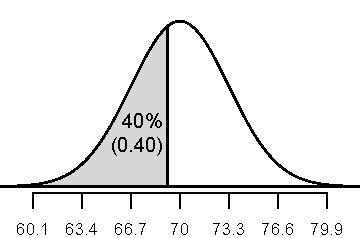
\includegraphics{lower40} % insert file ``lower40''
			% (in the same folder as this document)
			% no extension needed!

Basic figures are made using the \texttt{$\backslash$includegraphics} command. The size can also be controlled via the optional \texttt{space} argument.

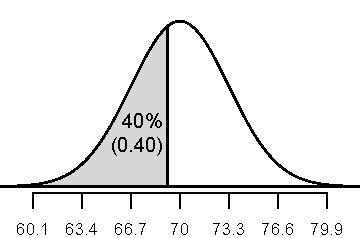
\includegraphics[height=1.0in]{lower40} % using the space option: [height=1.0in]

A figure can easily be centered in the same way a table was centered:
\begin{center}
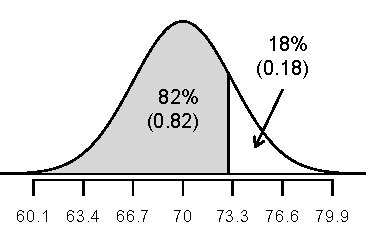
\includegraphics[height=1.0in]{figures/lower82/lower82}
\end{center}

\subsection{Captions and referencing}

Like tables, figures can also be ``floated'' and have captions/labels. The Templates give a nicer means to work with graphics. See Figure~\ref{figureTemplate}. Note that the Float Figure template from LaTeX does not include the space option, which you would need to add. \\
\begin{figure}[htbp]
	% as with floating tables, figures will float around the page and [htbp] offers some control
   \centering % one method to center the figure
   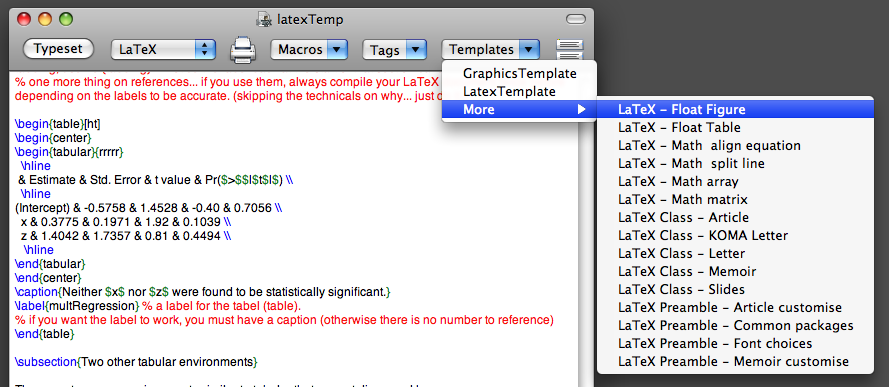
\includegraphics[height=2.0in]{figures/figureTemplate}
   	% notice that the figure was referenced in a folder
	% it is smart to manage your files carefully so not to make your 
	%	main folder messy
   \caption{Where to find your figure template.}
   \label{figureTemplate}
\end{figure}

\subsection{Keeping organized}

It is highly recommended that figures are organized into folders. This will keep the main folder from getting cluttered with lots of image files, like in Figure~\ref{messyFolder}. Figure~\ref{cleanFolder} shows a much better organization structure for the document figures. \\
\begin{figure}[htbp]
   \centering
   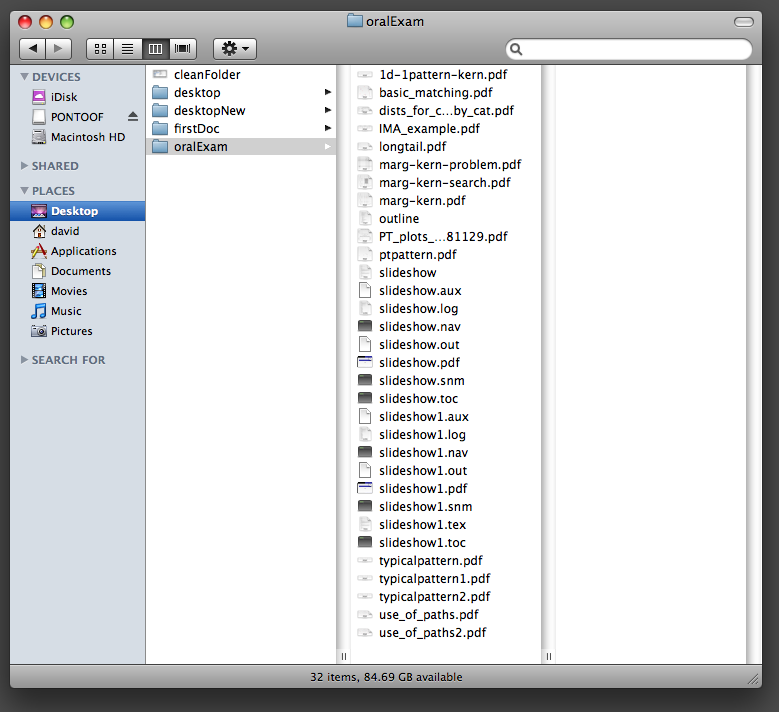
\includegraphics[height=3.0in]{figures/messyFolder}
   \caption{Don't do this. And name your files more carefully than this... ``slideshow'' is not specific.}
   \label{messyFolder}
\end{figure}
\begin{figure}[htbp]
   \centering
   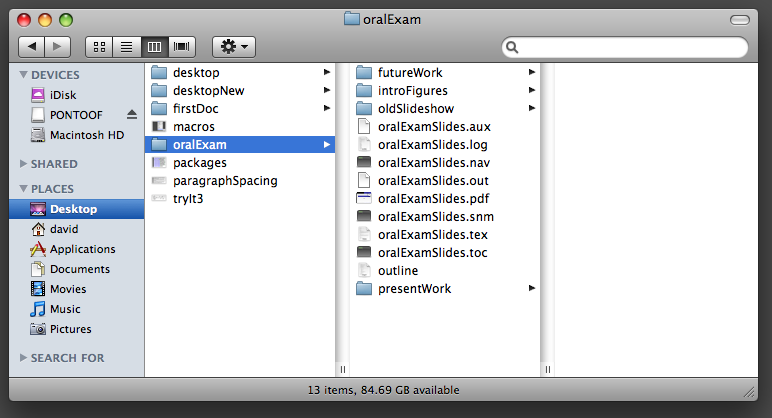
\includegraphics[height=1.8in]{figures/cleanFolder}
   \caption{Organize your files more like this.}
   \label{cleanFolder}
\end{figure}


\section{Math}
\label{math}

\subsection{Math in text}

LaTeX makes it easy to add Greek letters like $\alpha$, $\zeta$,
$\mu$, etc. into text. In the same way, equations can be added
easily as well: $y=x^3$, $\sum z^j$, $x_1+\cdots+x_n$.
\begin{center}
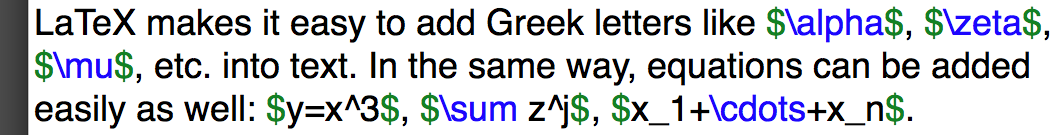
\includegraphics[height=1.5cm]{figures/mathInText}
\end{center}

Greek letters and math expressions such as $\alpha$, $\zeta$, $y=\sqrt{x}\log(x)$ can be inserted easily using two dollar signs; it's just a matter of remembering what the commands are for each math expression or symbol. For example, $\alpha$ is created using \texttt{\$$\backslash$alpha\$}. Based on how $\alpha$ was created, how would you think to create $\beta$?

The LaTeX and Matrix Panels have a large number of common symbols, letters, etc. and can be accessed by either \texttt{alt-command-[dash/underscore key]} or \texttt{alt-command-[+/= key]} in TeXShop or by navigating to them in the menu (see the ``Window'' menu in TeXShop). Some letters/symbols/etc that you can create... \\

$\hbar\imath\jmath\ell\Re\Im\emptyset\infty\partial\nabla\triangle\forall\exists\nexists\top\bot\dag\ddag\sum\prod\int\oint\bigcap\cap\bigcup\cup\biguplus\bigoplus\bigotimes\bigodot\hat{a}\bar{a}\tilde{a}$ \\

$\alpha\beta\gamma\delta\epsilon\varepsilon\zeta\eta\theta\iota\kappa\lambda\mu\nu\xi\pi\varpi\varrho
\sigma\varsigma\tau\upsilon\phi\varphi\chi\psi\omega$ \\

The number of available symbols is enormous. If you want the symbol, it probably exists in LaTeX. \\
% try looking in this (very big) PDF for what you want if you cannot find it in the LaTeX Panel:
%	www.ctan.org/tex-archive/info/symbols/comprehensive/symbols-a4.pdf


There are a huge number of ways to construct expressions...
\begin{eqnarray*} % we'll get to this new eqnarray environment in a moment...
\sqrt{2}, \quad \frac{5}{2+3}=1, \quad \left(\frac{5}{2+3}\right), \quad 2^10 \neq 2^{10} = 1024, \quad x_1 = 3 \\
\bar{x}, \quad 3 \geq x, \quad \lim_{x\to0}\left( \frac{\sin(x)}{x} \right) \to 1, \quad \frac{\sin(x)}{x}\stackrel{x\to0}{\to} 1
% \quad inserts a little space
% \frac has two arguments: the numerator and the denominator
% \left( and \right) make parenthesis that automatically adjust to fit the size of the inside expression, i.e. (\frac{5}{2+3}) doesn't look very nice
% ^ is used to make a superscript. in a similar way, _ is used for subscript
% when making super or subscripts, put them in parenthesis if it is more than a single character, e.g. x_{subscript} or x^{superscript}.
\end{eqnarray*}

\subsection{Equation environment and referencing}

Equations can also be put on their own line using the equation environment:
\begin{eqnarray}
A_{b_{ik}} % line breaks don't matter
		% make sure the use braces if subscripting more than a single character (otherwise it won't work...
		%	see 2^10 \neq 2^{10} = 1024 above
	= \sum_{l=1}^{k}\sum_{j=1}^{i} \gamma^{\alpha_{b_{jl}}}
\label{Abi}
\end{eqnarray}
Just like tables and figures, equations can also be referenced, such as Equation~\ref{Abi}. \\

If you do not want a number assigned to your equation, use the \texttt{eqnarray$^*$} environment:
\begin{eqnarray*}
A_{b_{ik}} = \sum_{l=1}^{k}\sum_{j=1}^{i} \gamma^{\alpha_{b_{jl}}}
\end{eqnarray*}
One more example below in Equation~\ref{powerSeries}...
\begin{eqnarray}
\sum_{k=0}^{\infty}0.5^k = \frac{1}{1-0.5} = 2
\label{powerSeries}
\end{eqnarray}


\subsection{Aligning}

If there is a multiline equation, then use two amperstands (\&) if any alignment is desired:
\begin{eqnarray*}
y &=& (x-b)^2 + a \\ % a double-backslash must be used to create a new line
&=& x^2 - 2bx + b^2 + a % the &'s around the equals signs on each line make them align
\end{eqnarray*}
If you don't use this, the alignment is usually poor.

\subsection{Arrays}

Arrays are easily constructed using the Matrix Panel:
\begin{eqnarray*}
\left(
	\begin{array}{ccc}
	\sigma_1^2 & \sigma_{1,2} & \sigma_{1,3} \\
	\sigma_{2,1} & \sigma_{2}^2 & \sigma_{2,3} \\
	\sigma_{3,1} & \sigma_{3,2} & \sigma_{3}^2
	\end{array}
\right)
\end{eqnarray*}
Array construction is essentally identical to tables, except now it is easy to insert mathematics.

\subsection{Some benefits of the package \texttt{amsmath}}

The package \texttt{amsmath} is not in the LaTeX template, however, it can be very handy.
If you have a longer equation and only want a number for one line, then use \texttt{$\backslash$notag}:
\begin{eqnarray}
&&Cov\left( \left(\bar{X}_{A}^{(k_1)} - \bar{X}_{B}^{(k_1)}\right)\sqrt{I_{k_1}}, \left(\bar{X}_{A}^{(k_2)} - \bar{X}_{B}^{(k_2)}\right)\sqrt{I_{k_2}} \right) \notag \\
&&\quad= Cov\left( \bar{X}_{A}^{(k_1)} - \bar{X}_{B}^{(k_1)}, \bar{X}_{A}^{(k_2)} - \bar{X}_{B}^{(k_2)}\right) \sqrt{I_{k_1}I_{k_2}} \notag \\ % \quad adds a little extra space
&&\quad= Cov\left( \bar{X}_{A}^{(k_1)} - \bar{X}_{B}^{(k_1)}, \bar{X}_{A}^{(k_2)} - \bar{X}_{B}^{(k_2)}\right) \sqrt{I_{k_1}I_{k_2}}
\end{eqnarray}
The package \texttt{amsmath} is required to use this command. This package is also required if text is added to an equation using \texttt{$\backslash$text}:
\begin{eqnarray*}
\bar{x} = \sum_{i=1}^{n} x_i \quad \text{and} \quad \hat{\sigma} = \sqrt{\frac{1}{n-1}\sum_{i=1}^n(x_i-\bar{x})^2}
\end{eqnarray*}
Another example of \texttt{eqnarray$^*$} with \texttt{$\backslash$text}:
\begin{eqnarray*}
\text{estimated time} = \frac{\text{distance of travel}}{\text{speed of the car}} + \text{any delays}
\end{eqnarray*}

\section{Practice}

Create a new document and produce the 3 items below. Be sure to update the \texttt{$\backslash$title} and \texttt{$\backslash$author} in your new document.

\subsection{Try it \#1}

Make the output shown in Figure~\ref{tryIt1} using the \texttt{tabular} environment.
\begin{figure}[htbp]
   \centering
   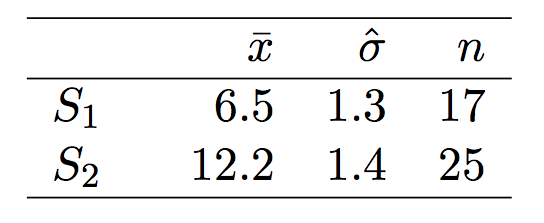
\includegraphics[height=0.8in]{tryIt/tryIt1}
   \caption{Try it \#1.}
   \label{tryIt1}
\end{figure}

\subsection{Try it \#2}

Make the following image 0.8 inches tall, center it, add a caption, and add a reference. Write a sentence referencing the figure (using \texttt{$\backslash$ref}) as well and compile your LaTeX document twice so the reference works. (If you use the Float Figure Template be sure to add the height option... alternatively, you might use an earlier LaTeX example as a template.) \\
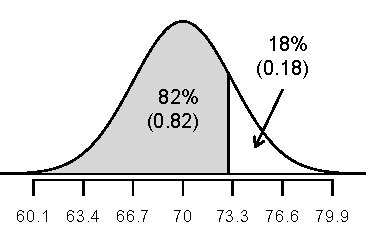
\includegraphics{figures/lower82/lower82}

\subsection{Try it \#3}

Produce the equation in Figure~\ref{tryIt3} using the \texttt{eqnarray$^*$} environment.
\begin{figure}[htbp]
   \centering
   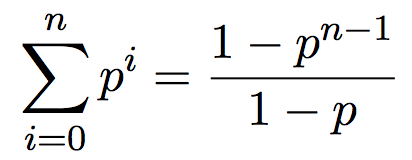
\includegraphics[height=0.5in]{tryIt/tryIt3}
   \caption{Try it \#3.}
   \label{tryIt3}
\end{figure}


\section{Bibliography stuff}

A point pattern is described as a realization of a point process \citep{daley}, and several one-dimensional distance functions for point patterns are described in \citet{victor}.

\bibliographystyle{biblio/simpleStyle}
\bibliography{biblio/bibDB}


\end{document}  